\begin{frame}[fragile]{Single-Sweep Reconstruction Maps and String-Method Locates Channels}
\begin{tikzpicture}[scaleall=1.0]
\pcuad{\textwidth}{\textheight}
%\showcuad
\path(nw) ++(-0.75,0.15) node(cites)[anchor=north west,text 
width=\textwidth]{{\tiny \textcolor{red!80!black}{
L. Maragliano, G. Cottone, G. Ciccotti, and E. Vanden-Eijnden, {\it JACS} {\bf 312}:1010 (2010)\\
M. Lapelosa and \underline{CFA}, {\it J Chem Theory Comput} {\bf 9}:1265 (2013)\\
A. Bucci and \underline{CFA}, {\it J Chem Theory Comput} {\bf 10}:2668 (2014)\\
}}};
\path(nw) ++(0.0,-0.75) node(cvtext) [anchor=north west,text width=\textwidth] {
$\thetab(\xb)\ :$\ center-of-mass  of O$_{\sf 2}$ in protein-fixed coordinate system.\\
$\Rightarrow$\ $P(\zb)$ = probability of finding O$_{\sf 2}$ at $\zb$ at equilibrium.};
\path(nw) ++(0.0,-2.5) node(pic) [graphics,anchor=north west]{
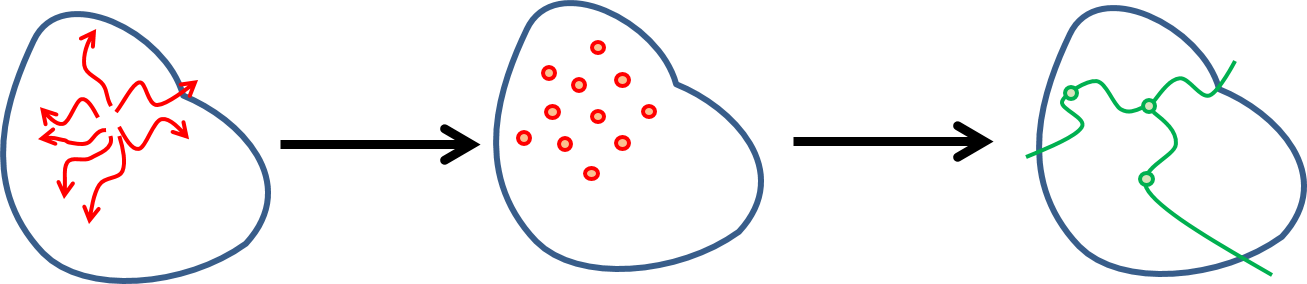
\includegraphics[width=\textwidth]{single_sweep_cartoon}};
\path(pic.south west) ++(-0.5,-0.25) node(tamdtext) [draw,anchor=north west,text width=0.3\textwidth] {
Use \textcolor{red}{TAMD} to enhance sampling of O$_{\sf 2}$ positions in protein and to identify all portals.};
\path(image) ++(-6.75,0.70) node(label1) [anchor=south west,text width=0.2\textwidth] { Downsample onto irregular 2.5-\AA\ mesh };
\path(tamdtext.north east) ++(0.5,0.0) node(restrainedMDtext) [draw,anchor=north west,text width=0.3\textwidth] {
Use \textcolor{green!80!black}{restrained MD} to compute mean force $f_i=\kappa\langle \thetab-\zb\rangle_{\zb_i}$ at each $\zb_i$};
\path(image) ++(-2.5,0.70) node(label1) [anchor=south west,text width=0.2\textwidth] { 
Use all $f_i$'s to construct $F(\zb)$ };
\path(restrainedMDtext.north east) ++(0.5,0.0) node(stringmethodtext) [anchor=north west,draw,text width=0.3\textwidth] {
Use steepest-descent and \textcolor{blue}{string method} to identify sites and pathways.};
\end{tikzpicture}
\end{frame}

